

A particularly interesting unitary to study is the DFT (Discrete Fourrier Transform), $(e^{\frac{i 2 k \pi j k}{m}})_{0 \leq j,k < m}$:
\[\Ufou = \begin{pmatrix}
            1 & 1 & \cdots & 1 \\
            \omega & \omega^{2} & \cdots & \omega^{m-1} \\
            \vdots \\
            \omega^{m-1} & \omega^{2(m-1)} & \cdots & \omega^{(m-1)^{2}} \\
          \end{pmatrix}\]

As we will see, this unitary is useful when decomposing other unitaries. It is therefor of interest to get sense for its effects. If we fix the input, simulate the fourrier unitary with a classical computer and plot all the output amplitudes we notice that this unitary exhibits symmetries that are not found in other matrices:

\begin{figure}[ht]
  \centering
  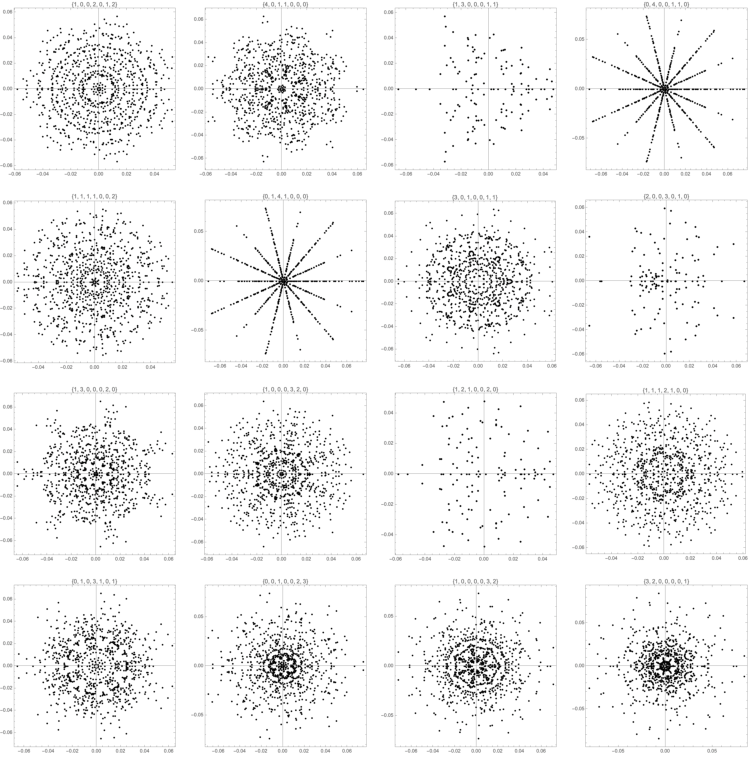
\includegraphics{figures/Mandalas.pdf}
  \caption{\label{fig:mandalas} Plots for various input histograms of the complex amplitudes of each output histogram. $N$ = 6, $m = 7$. }
\end{figure}

Further simulation suggests the following points:

\begin{itemize}
  \item There are families of histograms that give similar pictures.
  \item Most exhibit $m$-fold symmetry.
  \item Some less common families only exhibit $2$-fold symmetries.
\end{itemize}

We can investigate this using equation \ref{exp}. First we write the simplified expression for the specific unitary:

\begin{align*}
  \Ufou^{Q} &= \prod_{0 \leq i,j < m} \omega^{i \cdot j \cdot Q_{i,j}} \\
  &= \omega^{\sum_{0 \leq  i,j < m} i \cdot j \cdot Q_{i,j} \mod m}
\end{align*}

We are ready to study the simmetries. Let us fix an imput histogram: $ \vec{n} = (n_1,\cdots,n_{m})$. We consider an action of the dihedral group on this histogram. Recall that the dihedral group $D_{m}$ is the group of symmetries of a regular $m$-gon under rotations and reflections. It has the following presentation:

\[D_{m} = <r, s | s^{2} = \epsilon, srs = r^{-1}>\]

Where $r$ represents a unit rotation and $s$ a reflection. This group can acts on our histogram in the following way:

\begin{align*}
  r.(n_1, n_2, \cdots, n_{m}) &= (n_{m}, n_{1}, \cdots, n_{m-1}) \\
  s.(n_1, n_2, \cdots, n_{m}) &= (n_{m}, \cdots, n_{2}, n_{1}) \\
\end{align*}

Let us study the amplitude of output $\vec{n'}$ for a rotation: We notice that the matrices $Q$ that are compatible with $r.\vec{n}$ and $\vec{n'}$ are exactly the ones compatible with $\vec{n}$ and $\vec{n'}$ but with the lines rotated downwards, i.e. if we count the indices modulo $m$:

\begin{align*}
   \mathcal{A}_{\Ufou}(\vec{n'}, r.\vec{n}) &=  \sqrt{r.\vec{n}! \vec{n'}!} \sum_{Q \in \comp(r.\vec{n}, \vec{n'})} \frac{\omega^{\sum_{0 \leq  i,j < m} i \cdot j \cdot Q_{i,j}}}{Q!}\\
  &= \sqrt{\vec{n}! \vec{n'}!} \sum_{Q \in \comp(r.\vec{n}, \vec{n'})} \frac{\omega^{\sum_{0 \leq  i,j < m} i \cdot j \cdot Q_{i,j}}}{Q!}\\
  &= \sqrt{\vec{n}! \vec{n'}!} \sum_{Q \in \comp(\vec{n}, \vec{n'})} \frac{\omega^{\sum_{0 \leq  i,j < m} i \cdot j \cdot Q_{i,j+1}}}{Q!}\\
  &= \sqrt{\vec{n}! \vec{n'}!} \sum_{Q \in \comp(\vec{n}, \vec{n'})} \frac{\omega^{\sum_{0 \leq  i,j < m} i \cdot (j-1) \cdot Q_{i,j}}}{Q!}\\
  &= \sqrt{\vec{n}! \vec{n'}!} \sum_{Q \in \comp(\vec{n}, \vec{n'})} \frac{\omega^{\sum_{0 \leq  i,j < m} i \cdot j \cdot Q_{i,j}}\cdot \omega^{\sum_{0 \leq i,j < m} i Q_{i,j}}}{Q!}\\
  &= \sqrt{\vec{n}! \vec{n'}!} \sum_{Q \in \comp(\vec{n}, \vec{n'})} \frac{\omega^{\sum_{0 \leq  i,j < m} i \cdot j \cdot Q_{i,j}}\cdot \omega^{\sum_{0 \leq i < m} i n'_{i+1}}}{Q!}\\
  &= \omega^{\weight(\vec{n'})} \mathcal{A}_{\Ufou}(\vec{n'}, \vec{n})
\end{align*}

Where we define the weight of a histogram:\change{Maybe index from 0 everywhere}

\[\weight(\vec{n}) = 0 \cdot n_{1} + 1 \cdot n_{2} + \cdots + (m-1) \cdot n_{m-1} \mod m \]

The same type of cumputation gives:

\begin{align*}
  \mathcal{A}_{\Ufou}(\vec{n'}, s.\vec{n})   &= \omega^{\weight(\vec{n'})} \overline{\mathcal{A}_{\Ufou}(\vec{n'}, \vec{n})}
\end{align*}

This explains the plot families: within a given orbit of dihedral permutations, two input histograms will produce the exact same set of amplitudes, each shifted by a phase that depends on the weight of the corresponding \emph{output} histogram (and/or reversed along the real axis). The plots are then similar in that each of the $m$ weight classes gets shifted around by the same phase \ref{fig:weights}):\illustration{Would be nice to print the weight of each color}

\begin{figure}[ht]
  \centering
  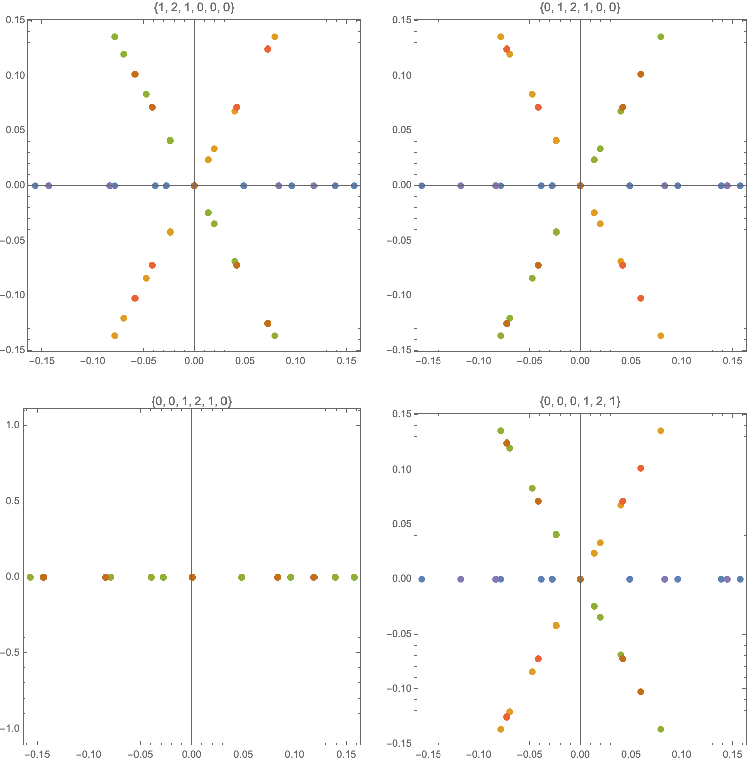
\includegraphics[scale=0.7]{figures/weights.pdf}
  \caption{\label{fig:weights} Here $N=4$, $m=6$, after each rotation the weight classes (each of a different color) get shifted by their own phase.}.
\end{figure}

We can also notice that the same reasonning applies to the output histogram:

\begin{empheq}[left = \empheqlbrace]{align*}
  \mathcal{A}_{\Ufou}(r.\vec{n'}, \vec{n})   &= \omega^{\weight(\vec{n})} \mathcal{A}_{\Ufou}(\vec{n'}, \vec{n}) \\
  \mathcal{A}_{\Ufou}(s.\vec{n'}, \vec{n})   &= \omega^{\weight(\vec{n})} \overline{\mathcal{A}_{\Ufou}(\vec{n'}, \vec{n})}
\end{empheq}

Which explains the presence of symmetries: most of the histograms studied have $m$-fold symmetry because in general the $m$ weight classes are evenly rotated, though in some cases (like the bottom left in \ref{fig:weights}) their phases line up and generate a pattern that looks sparser and less symmetric: many points overlap.
